%!TEX program = xelatex
\documentclass{beamer}

\usepackage[english]{babel}

\usepackage{graphicx,hyperref,url, materialbeamer}
\usepackage{braket}
%\usepackage{euler}
\usepackage{listings}

\setbeamercovered{transparent}


\usefonttheme{}

% The title of the presentation:
%  - first a short version which is visible at the bottom of each slide;
%  - second the full title shown on the title slide;
\title[FPAR]{First Person\\Action Recognition}

% Optional: a subtitle to be dispalyed on the title slide
\subtitle{Project Description}

% The author(s) of the presentation:
%  - again first a short version to be displayed at the bottom;
%  - next the full list of authors, which may include contact information;
\author[Nicolò Bertozzi, Francesco Bianco Morghet]{
  Nicolò Bertozzi, Francesco Bianco Morghet} 
  
%\titlegraphic{\includegraphics[width=\textwidth]{atac-logo}}

% The institute:
%  - to start the name of the university as displayed on the top of each slide
%    this can be adjusted such that you can also create a Dutch version
%  - next the institute information as displayed on the title slide
\institute[Politecnico di Torino]{
Machine Learning and Deep Learning\\
Master Degree in Data Science Engineering\\
Politecnico di Torino}

% Add a date and possibly the name of the event to the slides
%  - again first a short version to be shown at the bottom of each slide
%  - second the full date and event name for the title slide
\date[2$^{nd}$ Semester]{
 2$^{nd}$ Semester | 10 July 2020}

\providecommand{\di}{\mathop{}\!\mathrm{d}}
\providecommand*{\der}[3][]{\frac{d\if?#1?\else^{#1}\fi#2}{d #3\if?#1?\else^{#1}\fi}} 
 \providecommand*{\pder}[3][]{% 
    \frac{\partial\if?#1?\else^{#1}\fi#2}{\partial #3\if?#1?\else^{#1}\fi}% 
  }
\begin{document}

\begin{frame}
  \titlepage
\end{frame}

\begin{frame}
  \frametitle{Table of Contents}
  \tableofcontents
\end{frame}

\section{Introduction}

\begin{frame}
\frametitle{Overview} 
  \tableofcontents[currentsection]
\end{frame}

\begin{frame}
\frametitle{Introduction 1/4}
Goal:
\begin{itemize}
\item Record videos with the same cameraman's point of view;
\item Recognize the actions performed by the subject;
\end{itemize}
\end{frame}

\begin{frame}
\frametitle{Introduction 2/4}
\begin{columns}
\column{0.5\textwidth}
Interested Areas:
\begin{itemize}
\item Android intelligence;
\item Autonomous driving;
\item Surveillance;
\item Loyalizing users' experience;
\end{itemize}
\column{0.5\textwidth}
\begin{figure}
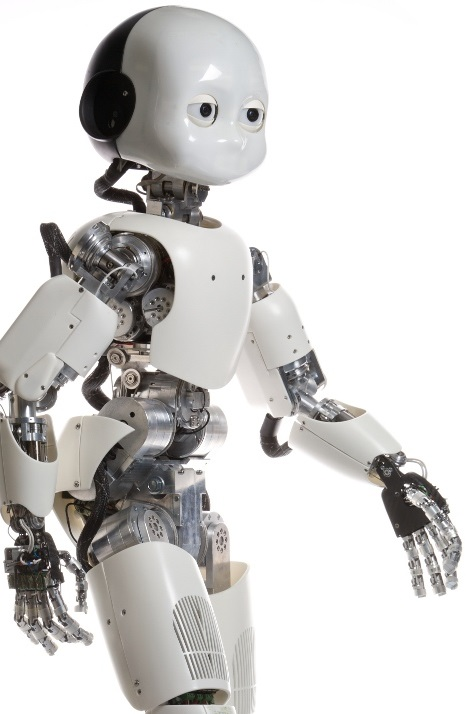
\includegraphics[width=0.8\textwidth]{../schemi/icub}
\end{figure}
\end{columns}
\end{frame}

\begin{frame}
\frametitle{Introduction 3/4}
Issues:
\begin{itemize}
\item Small datasets;
\item Presence of \textbf{parts of the cameraman's body} in the video;
\item The action \textbf{must be represented} by a \emph{verb + noun};
\end{itemize}
\end{frame}

\begin{frame}
\frametitle{Introduction 4/4}
Solutions:
\begin{itemize}
\item Sales of \textbf{wearable devices};
\item Incrementing chance of \textbf{having at hand a camera};
\item Incrementing number of \textbf{images taken every day} \cite{photos};
\item Deeper neural networks;
\end{itemize}
\end{frame}
      
\section{Related Works}

\begin{frame}
\frametitle{Overview} 
  \tableofcontents[currentsection]
\end{frame}

\begin{frame}
\frametitle{Two Stream Approach 1/2}
Main characteristics:
\begin{itemize}
\item Two \textbf{CNNs}: one to \textbf{extract features} from RGB images and one to \textbf{extract features} from flow images;
\item \textbf{ConvLSTM} to take into account the \textbf{temporal dependencies};
\item Linear \textbf{classifier} to \textbf{join the networks};
\end{itemize}
\end{frame}

\begin{frame}
\frametitle{Two Stream Approach 2/2}
Issue:
\begin{itemize}
\item The correlation and the \textbf{mutual influence} between motion and appearance information is \textbf{not taken into account};
\end{itemize}
Solution:
\begin{itemize}
\item Implementing a single network accompanied by a \textbf{motion segmentation task};
\end{itemize}
\end{frame}

\begin{frame}
\frametitle{Attention Map}
Features:
\begin{itemize}
\item \textbf{Focusing} the recognition on the \textbf{most important parts} of the video;
\item \textbf{Discarding} the regions with \textbf{low importance};
\item The temporal flow information, i.e \textbf{the motion}, \textbf{is not included} in the mechanism;
\end{itemize}
\end{frame}

\begin{frame}
\frametitle{Motion Segmentation Task}
Features:
\begin{itemize}
\item Each \textbf{feature map} is forwarded to an \textbf{auxiliary branch} with a convolutional and a FC layer;
\item \textbf{IDT} as ground truth: image which indicates if a \textbf{pixel is moving or not}, net to the camera motion;
\item \textbf{Pixel-per-pixel} loss between the predicted motion map and the IDT;
\end{itemize}
\end{frame}

\section{Proposed Methods}

\begin{frame}
\frametitle{Overview} 
  \tableofcontents[currentsection]
\end{frame}

\begin{frame}

\section{Proposed Methods}

\begin{frame}
\frametitle{Overview} 
  \tableofcontents[currentsection]
\end{frame}
     
\section{Conclusions}

\begin{frame}
\frametitle{Overview} 
  \tableofcontents[currentsection]
\end{frame}
     
\begin{frame}
\frametitle{References}
   \begin{thebibliography}{9}
	\bibitem{photos}
		Caroline Cakebread
		\newblock “People will take 1.2 trillion digital photos this year — thanks to smartphones”
		\newblock Businessinsider.com, 1 September 2017
		\newblock Available at: https://www.businessinsider.com/12-trillion-photos-to-be-taken-in-2017-thanks-to-smartphones-chart-2017-8?IR=T
   \end{thebibliography}
\end{frame}

\begin{frame}
\centering
\frametitle{The End}
\Huge Thank you for your attention!
\break
\break
\break
\break
\large Nicolò Bertozzi
\break
Francesco Bianco Morghet
\break
\break
FPAR Project | MLDL
\break
10 July 2020
\end{frame}
\end{document}